% Path diagram of the bivariate dual change score model (vignette lcs).
\documentclass[tikz, border = 6pt]{standalone}
\usepackage{amsmath}
\usepackage{bm}
\usetikzlibrary{arrows.meta, positioning, calc}
\tikzset{
  lat/.style = {circle, draw, thick, minimum size = 12mm, inner sep = 0pt},
  obs/.style = {rectangle, draw, thick, minimum size = 10mm, inner sep = 1pt},
  noise/.style = {circle, draw, minimum size = 7mm, inner sep = 0pt},
  reg/.style = {-{Stealth[length = 2.5mm]}, thick},
  cov/.style = {{Stealth[length = 2mm]}-{Stealth[length = 2mm]}},
  lab/.style = {font = \footnotesize, fill = white, inner sep = 1pt},
  dots/.style = {font = \Large}
}
\begin{document}
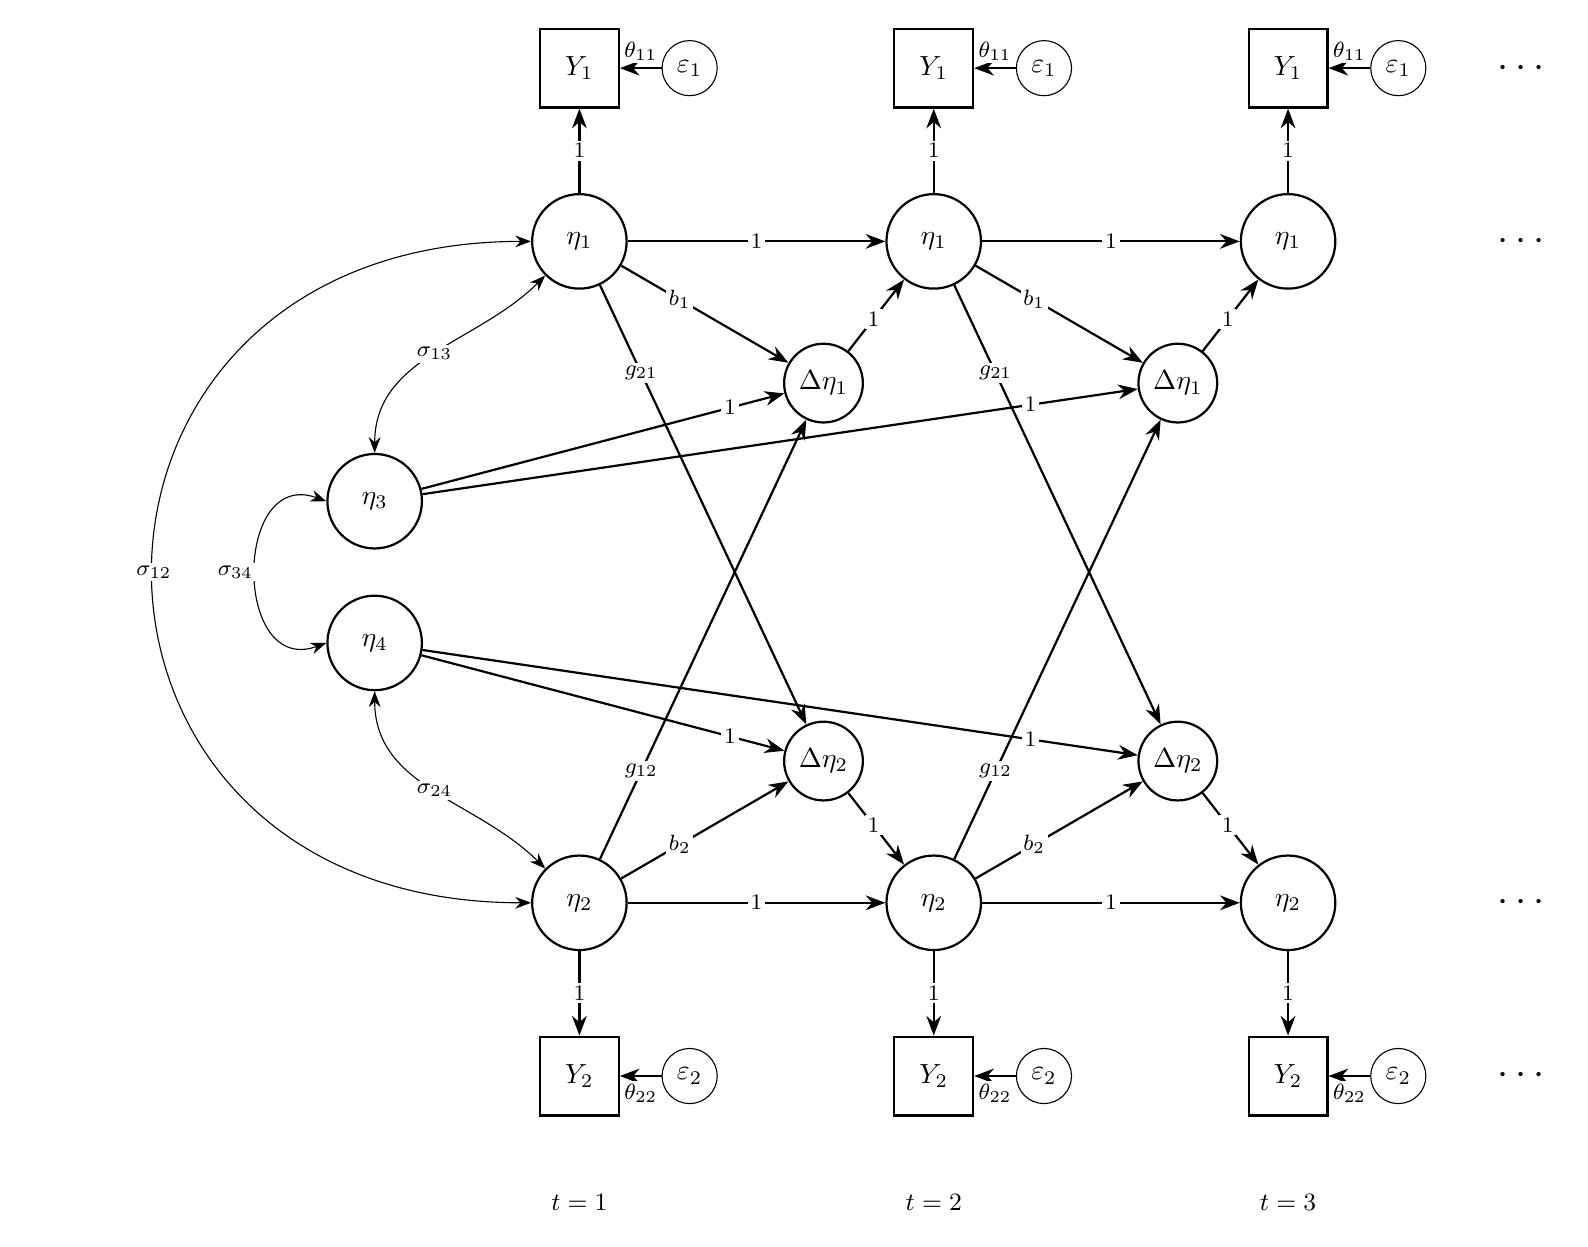
\begin{tikzpicture}[chg/.style = {circle, draw, thick, minimum size = 10mm, inner sep = 0pt}]
  % occasions
  \foreach \t/\x in {1/0, 2/4.5, 3/9} {
    \node[lat] (a\t) at (\x, 4.2) {$\eta_{1}$};
    \node[lat] (b\t) at (\x, -4.2) {$\eta_{2}$};
    \node[obs] (ya\t) at (\x, 6.4) {$Y_{1}$};
    \node[obs] (yb\t) at (\x, -6.4) {$Y_{2}$};
    \node[noise] (ua\t) at (\x + 1.4, 6.4) {$\varepsilon_{1}$};
    \node[noise] (ub\t) at (\x + 1.4, -6.4) {$\varepsilon_{2}$};
    \draw[reg] (a\t) -- node[lab] {1} (ya\t);
    \draw[reg] (b\t) -- node[lab] {1} (yb\t);
    \draw[reg] (ua\t) -- node[lab, above = 0.5mm] {$\theta_{11}$} (ya\t);
    \draw[reg] (ub\t) -- node[lab, below = 0.5mm] {$\theta_{22}$} (yb\t);
    \node[font = \small] at (\x, -8) {$t = \t$};
  }
  % slopes
  \node[lat] (s1) at (-2.6, 0.9) {$\eta_{3}$};
  \node[lat] (s2) at (-2.6, -0.9) {$\eta_{4}$};
  % latent change scores
  \foreach \s/\t/\x in {1/2/4.5, 2/3/9} {
    \node[chg] (da\t) at (\x - 1.4, 2.4) {$\Delta \eta_{1}$};
    \node[chg] (db\t) at (\x - 1.4, -2.4) {$\Delta \eta_{2}$};
    \draw[reg] (a\s) -- node[lab, pos = 0.5] {1} (a\t);
    \draw[reg] (b\s) -- node[lab, pos = 0.5] {1} (b\t);
    \draw[reg] (da\t) -- node[lab, pos = 0.45] {1} (a\t);
    \draw[reg] (db\t) -- node[lab, pos = 0.45] {1} (b\t);
    \draw[reg] (a\s) -- node[lab, pos = 0.35] {$b_{1}$} (da\t);
    \draw[reg] (b\s) -- node[lab, pos = 0.35] {$b_{2}$} (db\t);
    \draw[reg] (b\s) -- node[lab, pos = 0.2] {$g_{12}$} (da\t);
    \draw[reg] (a\s) -- node[lab, pos = 0.2] {$g_{21}$} (db\t);
    \draw[reg] (s1) -- node[lab, pos = 0.85] {1} (da\t);
    \draw[reg] (s2) -- node[lab, pos = 0.85] {1} (db\t);
  }
  % initial condition
  \draw[cov] (a1.west) .. controls (-7, 4.2) and (-7, -4.2) ..
    node[lab, pos = 0.5] {$\sigma_{12}$} (b1.west);
  \draw[cov] (s1.west) to[out = 160, in = 200, looseness = 1.8]
    node[lab, left] {$\sigma_{34}$} (s2.west);
  \draw[cov] (a1.south west) to[out = 225, in = 90]
    node[lab] {$\sigma_{13}$} (s1.north);
  \draw[cov] (b1.north west) to[out = 135, in = -90]
    node[lab] {$\sigma_{24}$} (s2.south);
  \foreach \rr in {6.4, 4.2, -4.2, -6.4} {
    \node[dots] at (12, \rr) {$\cdots$};
  }
\end{tikzpicture}
\end{document}
